\section{Introduction}
\label{sec:intro}
The CMS Collaboration has reported results of searches in the final states with two same-sign isolated leptons,
jets and missing energy~\cite{sspaper2010,ssnote2011,sspaper2011},
including a more specific search targeting the same-sign top pair production~\cite{sstop}.
The major background in all these analyses is from \ttbar\ production, as shown in Fig.~\ref{fig:ttbar}.

\begin{figure}[htb]
\begin{center}
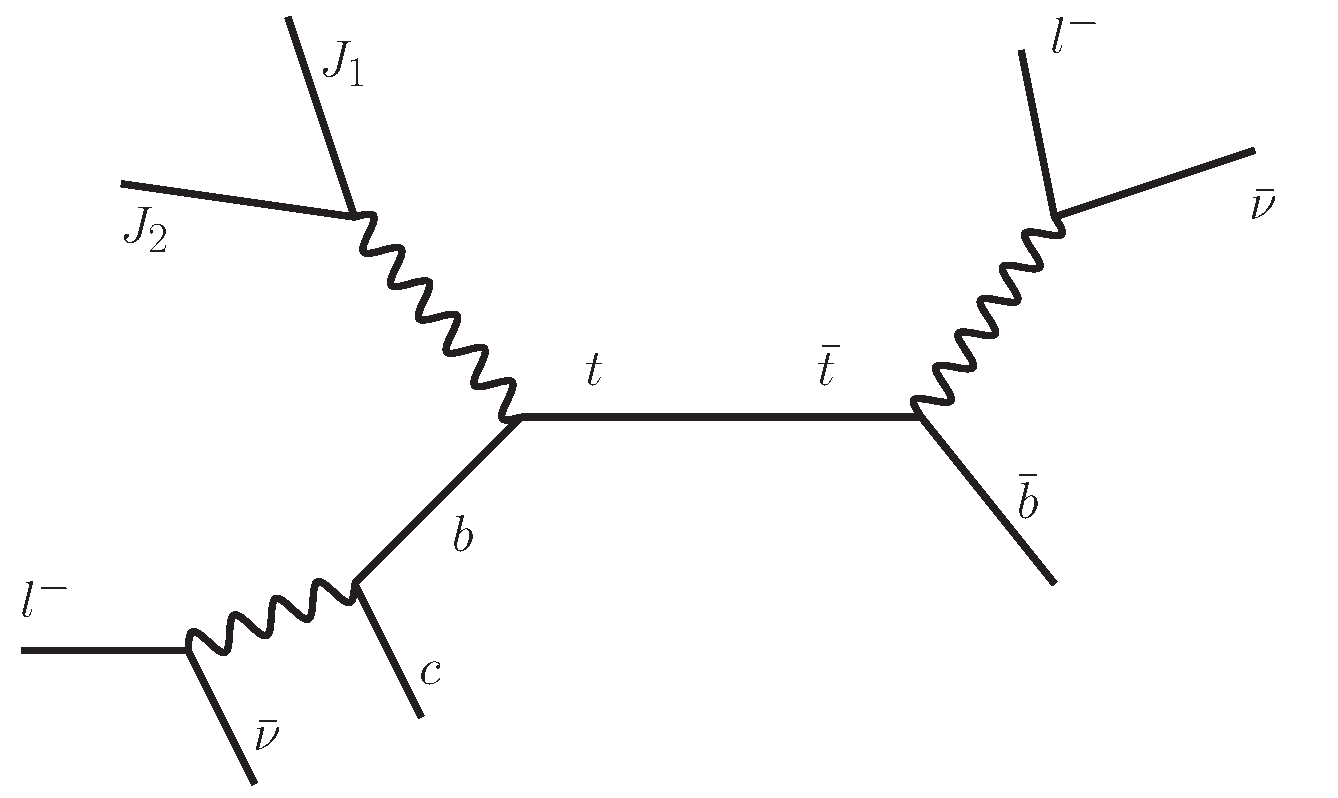
\includegraphics[width=0.6\linewidth, height=0.35\linewidth]{figs/ttbar.pdf}
\caption{ Diagram for \ttbar\ decays giving rise to same-sign dilepton final states \label{fig:ttbar}}
\end{center}
\end{figure}

The dominant source of same-sign dileptons in \ttbar\ 
are events where 
one of the leptons is from $W \rightarrow \ell \nu $ and the other originates from semi-leptonic $b$ decays. 
We refer to the first as ``real lepton'' and the second as ``fake lepton''.
An additional requirement on the number of $b$ jets $\geq 2$, 
reduces this background significantly,
as a b-quark cannot produce an isolated lepton and at the same time 
provide a b-tag.  In other words, the two b-quarks in a top event
cannot give three distinct, well separated objects: two tagged jets
and one isolated lepton.

Same-sign dileptons in association with two or more b-quarks appear naturally in many new physics scenarios.
They have been proposed as signatures of supersymmetry 
(SUSY) where heavy flavor (top or bottom) jets appear naturally~\cite{naturalness1,naturalness2,naturalness3,naturalness4},
in particular in processes with virtual stop contributions~\cite{stopVirtual,stopVirtualPRD},
those with resonant stop~\cite{stopReal},
all alternatively described with simplified models (SMS)~\cite{wacker}; 
%sbottom,gluinosbottom,
color-octet scalar production (either as sgluons in the context of SUSY~\cite{sgluons},
or non-SUSY in the context of minimal flavor violation~\cite{colorOctetScalars}); 
models of maximal flavor violation (MaxFV)~\cite{mxflv1,mxflv2,mxflv3}; 
same-sign top quark production from flavor changing neutral currents in the top sector~\cite{fcnczprime};
pair production of $T_{5/3}$~\cite{t53};
and top compositeness~\cite{topcomp1,topcomp2,topcomp3}
%this should go into refs for susy: pair production of scalar gluons~\cite{},
among others.

As was done in References~\cite{sspaper2010},\cite{ssnote2011},
and~\cite{sspaper2011}, we present our results in such a way that 
they can (reletively) easily be used by phenomenologists to
confront any model of new physics that produces same-sign 
dileptons, $b$-jets, and missing energy.

In addition, among all potential new physics models 
we select the following to report the sensitivity of this analysis:
\begin{enumerate}
\item the same-sign top pair production via $Z^\prime$~\cite{sstop,fcnczprime};

\item the same-sign top pair production in MaxFV~\cite{mxflv3};

\item $\ttbar \ttbar \widetilde\chi_1^0\widetilde\chi_1^0$ final state via (exclusive) gluino pair production with 
each gluino decaying a top-stop pair and the stop decaying
exclusively to top and LSP, all on-shell;

\item $\ttbar \ttbar \widetilde\chi_1^0\widetilde\chi_1^0$ final state via (exclusive) gluino pair production with 
each gluino decaying to a \ttbar\ and LSP 
via a virtual stop exchange\cite{T1tttt}; 
this decay mode of the gluino would dominate 
if all squarks were very massive with the stop being the lightest;
\item $\ttbar W^+W^- \chi_1^0\chi_1^0 $ final state via (exclusive) sbottom pair production with each 
sbottom decaying to a top and the lightest chargino, which subsequently decays to a W boson and an LSP;
\item a mix of $\ttbar b\bar{b} W^+W^- \widetilde\chi_1^0\widetilde\chi_1^0 $ and 
  $tt\bar{b}\bar{b}W^-W^-\tilde{\chi}_1^0\tilde{\chi}_1^0$ (+c.c.) final states via (exclusive) gluino pair or gluino-sbottom
  production where each gluino decays to a sbottom and a b-quark and the sbottom subsequently decays as
  $\widetilde{b} \to t \widetilde{\chi}^-_1 \to t W^- \widetilde{\chi}^0_1  $, as in the previous case.
\end{enumerate}
The considered models thus have two to four b-jets, and two to four W bosons in the final state with varying kinematics.

All of these new physics scenarios have in common that the isolated same-sign leptons are typically decay products of on-shell W's,
thus allowing us to increase the minimum lepton $p_T$ 
requirements in our search to 20~\GeV, which reduces backgrounds even further
with respect to the analysis of Ref.~\cite{sspaper2010,ssnote2011,sspaper2011}.
The combination of requiring at least two $b$ jets and increasing the lepton $p_T$ threshold to 20~\GeV\ reduces the standard model backgrounds
by roughly a factor 30 over the more generic search.
%%% ~\cite{sspaper2010,sspaper2011}.


%In this note we perform an inclusive signature based search for events with two isolated, same-sign leptons,
%in association with at least 2 $b$ jets and \met. This generic signature should be sensitive to 
%a wide variety of new physics scenarios leading to one or more same-sign top pairs in the final state, as well as the standard model
%production of $t\bar{t}W$. In addition to the inclusive search, we thus perform several dedicated searches for a variety
%of physics scenarios, including the standard model production of $t\bar{t}W$.
 
For the purpose of this note we restrict ourselves to the $ee$, $e\mu$, and $\mu\mu$ 
final states, {\em i.e.}, we do not consider $\tau$'s, except in the case that the $\tau$ decays leptonically.

This note is organized as follows.
A brief description of the event baseline selections is given in Section~\ref{sec:eventsel},
followed by the definitions of the signal search regions in Section~\ref{sec:regions}.
Estimates of efficiencies for leptons, \met, \Ht, and b-tags, components of the event selection,
are given in Section~\ref{sec:seleff}.  This can be used to provide
informaton to non-CMS members to better interpret our results (the so-called
``outreach'' program).
Data - Monte Carlo scale factors and their uncertainties are described
in Section~\ref{sec:SF}; these scale factors are needed to 
calculate signal acceptances.
% set limits on various models.
We then describe methods to predict background contributions in Section~\ref{sec:bkgds},
including predictions from simulation and from data, detailed in Section~\ref{sec:datadriven}.
Results of background predictions for the defined search regions are compared with 
observed events in data in Section~\ref{sec:yields},
supported by an exclusive (disjoint) breakdown of contributions in Appendix~\ref{sec:yields_exclusive}.
Comparisons of the predicted and observed events, together with inputs relevant
to signal selection systematic uncertainties described in Section~\ref{sec:systematic}.  Supporting information for the outreach program, {\it e.g.},
a validation of the efficiency model, is given in Section~\ref{sec:outreach}.
Finally, we interpret our findings as upper limits on 
production of signal events beyond
the background predictions as described in Section~\ref{sec:stampCollecting}.






